\chapter{Validazione}
\label{ch:validazione}

In questo capitolo verranno presentati i risultati relativi ai test effettuati utilizzando entrambi gli approcci implementati (l'approccio BLE Mesh e l'approccio BLE Mesh con il supporto della tecnologia Wi-Fi). Oltre a presentare i risultati ottenuti, verrà descritto lo scenario di test e la descrizione delle metriche impiegate al fine di analizzare i dati acquisiti. I parametri che verranno analizzati sono la \textit{letency}, il \textit{goodput} e il \textit{pdr}.

\section{Scenario}
Lo scenario in cui verrà valutato l'intero progetto riguarderà un ambiente indoor in un contesto urbano. Poiché il contesto abitativo riguarda una casa piuttosto isolata con limitate attività in sua prossimità, si avrà uno scenario soggetto a limitate interferenze, sulla frequenza trasmissiva, dell'ambiente circostanze. Lavorando in uno scenario del genere, le perdite di pacchetti verificate riguarderanno solo l'elevato carico di lavoro della rete e lievemente le infrastrutture circostanti (reti Wi-Fi o altri dispositivi operandi nella frequenza 2,4 GHz).\\

\noindent Al fine di eseguire delle analisi in modo accurato sul comportamento dell'intera rete mesh indoor, prima di procedere con l'esecuzione dei test (approccio solo BLE Mesh e approccio BLE Mesh con Wi-Fi) è stato necessario posizionare i nodi ad una distanza tale per cui ogni nodo risultasse in grado di comunicare solo ed esclusivamente con un vicino adiacente (nodo in sua prossimità). L'individuazione dei punti in cui posizionare i nodi è stata individuata analizzando il raggio di comunicazione, nello specifico analizzando il \texttt{TTL} contenuto nei messaggi scambiati all'interno della rete.\\ 
Ogni nodo, avente la funzione di \textit{relay}, alla ricezione di un messaggio non destinato a sé stesso procede in primo luogo a decrementare il campo \texttt{TTL} e successivamente, se tale valore risulta maggiore di 1, procede con l'inoltro.\\
A seguito di tale analisi ogni nodo è stato posizionato ad una distanza di circa $6m$ dal suo vicino, così come mostrato dalla figura \nameref{fig:rete_mesh}. In questo modo un messaggio per giungere da un'estremità all'altra della rete dovrà attraversare tutti i nodi di cui essa risulta essere composta, evitando così anche la circolazione di messaggi duplicati all'interno della rete.

\begin{figure}[!ht]
    \centering
    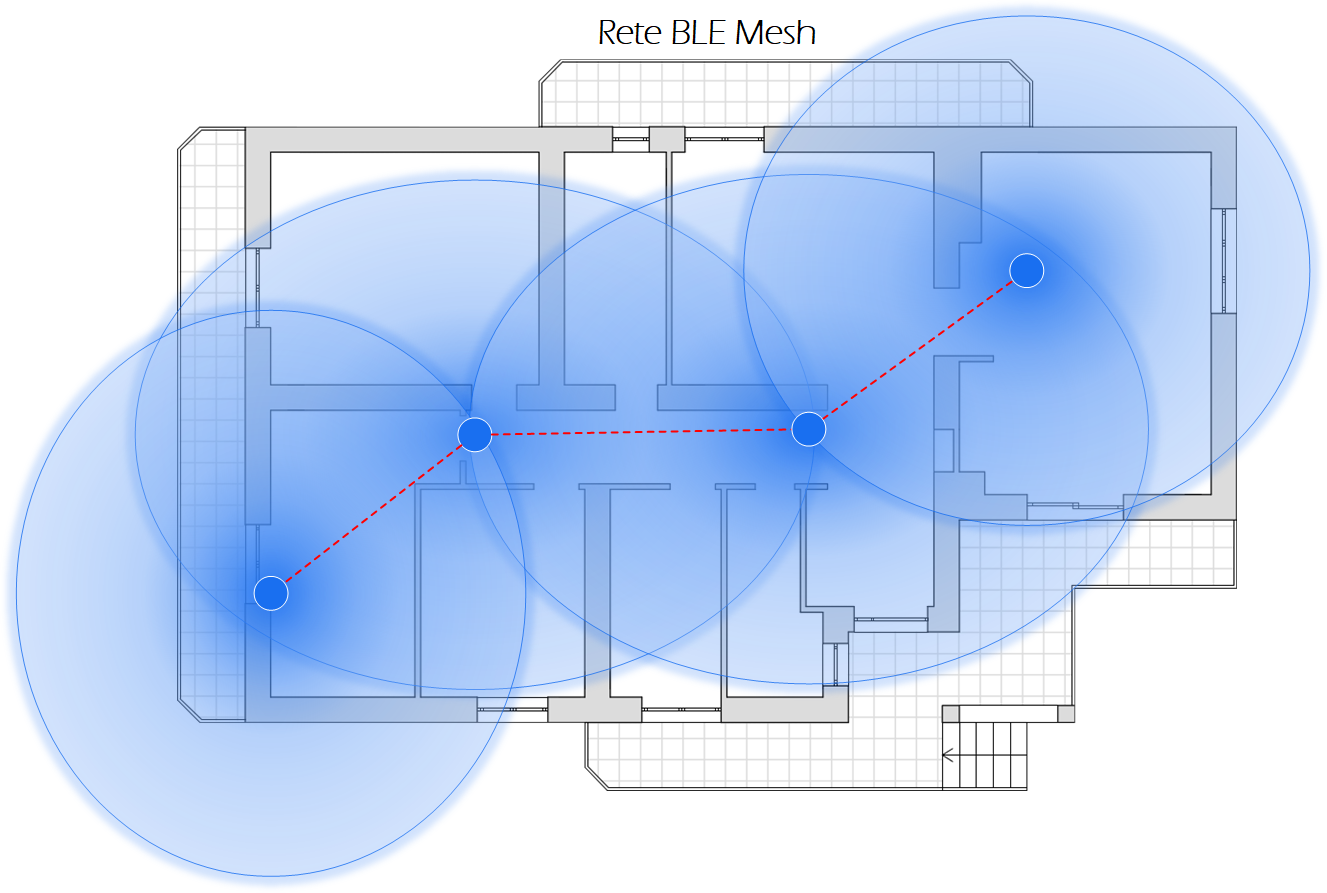
\includegraphics[width = 0.95\textwidth]{images/Rete_mesh_.png}
    \caption{Posizione dei nodi durante un test relativo alla \texttt{Configurazione 3}}
    \label{fig:rete_mesh}
\end{figure}

\noindent Al fine di studiare il comportamento della rete, utilizzando i due approcci descritti nei capitoli precedenti, sono stati definiti dei test in funzione alla distanza tra mittente e destinatario e all'aumentare del carico di lavoro.\\
Il variare della distanza ha portato alla definizione di tre configurazioni.
\begin{itemize}
    \item la configurazione \texttt{1} prevede l'impiego di due dispositivi soltanto (\texttt{Switch} e \texttt{Node-3}).
    \item la configurazione \texttt{2} prevede l'impiego di tre dispositivi. Il destinatario è stato posto ad una distanza maggiore e per garantire la comunicazione è stato necessario introdurre il nodo \texttt{relay-1}.
    \item la configurazione \texttt{3} prevede l'impiego di quattro dispositivi. Il destinatario è stato distanziato ulteriormente e quindi è stato necessario introdurre \texttt{relay-2} per garantire la comunicazione.
\end{itemize}

\noindent Il variare del carico di lavoro è stato gestito modificando la frequenza con cui i messaggi vengono immessi nella rete.
In tale circostanza sono stati presi in considerazione i seguenti periodi: \texttt{\textit{50ms}}, \texttt{\textit{100ms}}, \texttt{\textit{150ms}}, \texttt{\textit{200ms}}, \texttt{\textit{250ms}}, \texttt{\textit{500ms}} e \texttt{\textit{1000ms}}.\\
Il \textit{periodo} (\textit{T}), misurato in \textit{s}, è quella grandezza fisica che misura l'intervallo di tempo tra gli istanti iniziali di due eventi successivi.
La \textit{frequenza} (\textit{f}), misurata in \textit{Hz}, è quel fenomeno fisico che presenta un andamento costituito da eventi che si ripetono identici o quasi identici nel tempo e viene definita dal numero degli eventi che si ripetono in una data unità di tempo. Poiché la frequenza consente di esprimere meglio in concetto in merito al carico di lavoro della rete e può essere calcolata come l'inverso del periodo tramite la formula:
$$ f = \frac{1}{T} $$
si ottengono i seguenti valori (riportati nel medesimo ordine con cui sono stati espressi i periodi): \texttt{\textit{20 Hz}}, \texttt{\textit{10 Hz}}, \texttt{\textit{6.67 Hz}}, \texttt{\textit{5 Hz}}, \texttt{\textit{4 Hz}}, \texttt{\textit{2 Hz}} e \texttt{\textit{1 Hz}}.\\


\noindent Al fine di ottenere dei dati significativi per potere eseguire della analisi statistiche accurate, il test per ogni terna creata combinando \textit{configurazione}, \textit{frequenza} e \textit{approccio} hanno avuto una durata di \texttt{5} minuti e ripetuti \texttt{5} volte. Per garantire la medesima durata di ogni esperimento eseguito e allo stesso tempo avere carichi di lavoro ben distinti, il numero di messaggi inviati risulta essere inversamente proporzionane alla frequenza utilizzata.\\

\noindent L'insieme di tutti i test effettuati, ha comportato così una durata di circa 1050 minuti, ovvero circa \texttt{18} ore.

\section{Metriche}

\subsubsection{Latency}
La latenza, detta anche \textit{delay}, indica il tempo impiegato da una richiesta per passare dal mittente al ricevente e comprende anche il tempo impiegato dal destinatario per l'elaborazione del messaggio. La latenza in una rete è misurata in millisecondi e può essere misurata come il Round Trip Time (\texttt{RTT}) tra il client e il server. L'\texttt{RTT} o tempo di andata e ritorno, indica la durata, espressa in millisecondi (ms), necessaria affinché un pacchetto passi da un punto di partenza (mittente) ad uno di destinazione e nuovamente al punto di partenza. L'\texttt{RTT} è una metrica importante nel determinare lo stato di una connessione, al fine di diagnosticare la velocità e l'affidabilità delle connessioni di rete.\\
Tale valore è ottenuto mediante la differenza tra il tempo acquisito alla trasmissione del pacchetto (\texttt{start\_time}) e il tempo acquisito alla ricezione della relativa risposta (\texttt{final\_time}). Con tale calcolo otteniamo il \texttt{RTT}, mentre per determinare la latenza della rete, tale valore è stato ripartito per la fase di invio e la fase di ricezione, ovvero brutalmente diviso per due.
$$ latency = \frac{final\_time - start\_time}{2} $$

\subsubsection{Goodput}
Il Throughput misura la quantità di pacchetti scambiati (consegnati con successo) sulla rete, in un certo intervallo di tempo, al fine di determinare l'efficienza di tale rete. Il Goodput può essere definito come il Throughput a livello applicativo di una comunicazione. Ovvero, il numero di informazioni utili (misurate in bit) consegnate dalla rete ad una certa destinazione per unità di tempo.\\
La quantità di dati presi in considerazione comprende solo il Payload del messaggio, escludendo l'overhead richiesto dal protocollo per gestire l'intera trasmissione del pacchetto.\\
L'indice è calcolato dividendo la quantità di dati trasmessi con successo nell'unità di tempo. Non rientrano in questo conteggio i segmenti trasmessi con errore o duplicati. Il risultato viene rappresentato in Bps (Byte per second).
$$ goodput = \frac{pkt\_num \times pkt\_size}{time} $$

\noindent In cui \texttt{pkt\_num} indica il numero di pacchetti ricevuti correttamente durante l'intero test, \texttt{pkt\_size} indica la dimensione dell'informazione utile scambiata e \texttt{time} indica il tempo necessario alla ricezione di tutti i messaggi spediti.\\
Poiché con un payload superiore ad 11 byte il Lower Transport Layer prevede la segmentazione del pacchetto, la dimensione scelta risulta essere nettamente inferiore e legata al modello utilizzato (\texttt{Generic Level Set}). In tale circostanza l'informazione utile, ovvero lo \texttt{STATUS} dell'elemento è rappresentato impiegando 2 byte.

\subsubsection{Packet Delivery Ratio}
Il Packet Delivery Ratio (\texttt{PDR}) indica il tasso tra il numero di pacchetti ricevuti e il numero di pacchetti inviati attraverso la rete. 
$$ PDR = \frac{\sum packet\_received}{\sum packet\_sent} $$

\subsubsection{Intervalli di confidenza}
I risultati ottenuti utilizzando le metriche sopra descritte sono accompagnati da un intervallo di confidenza al fine di rendere precisa la stima del campione riportata.\\
L'intervallo di confidenza fornisce informazioni riguardo alla precisione dei valori ottenuti attraverso lo studio del campione. \\
Si è ricorso al calcolo dell'intervallo di confidenza poiché, la stima puntuale fornisce un valore singolo che varia a seconda del campione e difficilmente coincide con il valore vero della popolazione. Impiegando tale stima è possibile fornire un insieme di valori (un intervallo) che con una certa ``confidenza'' contiene il valore vero della popolazione.\\
In tale circostanza è stato calcolato un intervallo di confidenza del 95\%, in modo da affermare con una margine di certezza ragionevole (appunto 95\%) che quell'intervallo conterrà il valore vero dell'intera popolazione.\\

\noindent L'intervallo di confidenza al 95\% lo si ottiene mediante le seguente formule:
$$\bar{x} = \frac{\sum x}{n}$$
$$\sigma = \sqrt{\frac{\sum (x-\bar{x})^2}{n}}$$
$$\bar{x} \pm Z_{\alpha/2} \times \frac{\sigma}{\sqrt{n}}$$

\noindent in cui nella prima formula: $\bar{x}$ indica la media aritmetica della metrica in esame, $n$ indica la numerosità del campione e in tale circostanza coincide con il numero di run eseguiti per ogni tipologia di test (ovvero 5 run). La seconda formula consente di calcolare la deviazione standard (il grado di dispersione della distribuzione) ed indicata con la lettera greca sigma ($\sigma$). Le prime due formule sono impiegate nella terza formula per definire l'intervallo di confidenza, dove il simbolo $\pm$ permette il calcolo del limite inferiore e superiore dell'intervallo e $Z_{\alpha/2}$ indica il coefficiente di confidenza (poiché è stato scelto di calcolare l'intervallo di confidenza al 95\% tale valore coincide con $1.96$).

\subsubsection{Consumi Energetici}
La scelta di impiegare maggiormente la tecnologia Bluetooth è legata principalmente, come anticipato nei precedenti capitoli, i consumi energetici. I valori di riferimenti sono stati presi dalla documentazione ufficiale rilasciata da \texttt{Espressif} \cite{datasheet2019line}. In cui si afferma che i consumi per la trasmissione di un messaggio impiegando la tecnologia Bluetooth sono di 130 mA, mentre impiegando la tecnologia 802.11b i consumi risultano essere nettamente più elevati, ovvero arriviamo a 230 mA.

\section{Risultati}
In questa sezione vengono analizzati i risultati ottenuti in rispetto dei requisiti stabiliti e riguardanti le tre metriche precedentemente descritte.\\
I dati sono stati analizzati utilizzando degli script \texttt{python} in grado di acquisire le informazioni memorizzate nei file di log durante l'esecuzione dei test, ripulire i dati acquisiti, rimuovere il transiente iniziale (fase necessaria alla rete per giungere a pieno regime) in modo da analizzare il comportamento della rete quando risulta essere a pieno regime. Una volta ripuliti i dati secondo quanto descritto, sono stati elaborati utilizzando le suddette metriche ed infine generati i seguenti grafici per facilitare la comprensione del comportamento della rete mesh nelle varie situazioni.

\subsubsection{Risultati Bluetooth Mesh}
\noindent Con il seguente grafico relativo all'impiego della sola tecnologia Bluetooth Mesh, si vuole mostrare come la rete, con l'aumentare del carico di lavoro e con l'incrementare del numero di nodi intermedi frapposti tra mittente e destinatario, tende a diminuire di prestazione.\\

\noindent Un lieve calo prestazionale si intravede sin da subito ed è legato all'aumentare della distanza tra mittente e destinatario il che comporta ai pacchetti di dover attraversare dei nodi intermedi prima di giungere a destinazione. La relazione tra frequenza e prestazione della rete è inversamente proporzionale, come era prevedibile. Vale a dire che all'aumentare della frequenza di trasmissione, la prestazione della rete tende a diminuire.

\begin{figure}[hbt!]
    \centering
    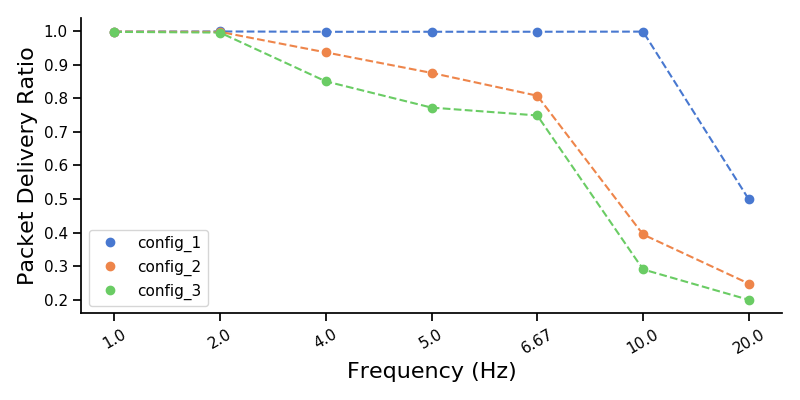
\includegraphics[width = 0.95\textwidth]{images/graphs/ble_pdr.png}
    \caption{Packed Delivery Ratio - Bluetooth Mesh}
    \label{graph:ble_pdr}
\end{figure}

\noindent Il punto in cui si evince così tanta differenza, per le \texttt{conf\_2} e \texttt{conf\_3}, riguarda l'impiego dei seguenti tassi trasmissivi: \texttt{150ms} (6.67 Hz) e \texttt{100ms} (10 Hz); mentre per la \texttt{conf\_1} tale situazione si verifica con l'impiego dei tassi trasmissivi: \texttt{100ms} (10 Hz) e \texttt{50ms} (20 Hz). \\
In quest'ultima circostanza il calo delle prestazioni è legato non solo al carico di lavoro che deve gestire la rete ma anche ai limiti imposti dalla tecnologia utilizzata. Per sopperire a tali perdite prestazionali si è fatto ricorso ad una tecnologia di supporto impiegata come descritto nei capitoli precedenti.\\

\noindent In merito alla \textit{latenza}, si può notare una variazione costante a partire dall'invio di messaggi ogni \texttt{150 ms}. La quale tende a raddoppiare nel momento in cui si passa da \texttt{conf\_2} a \texttt{conf\_3}. Analizzando più accuratamente il seguente grafico, si può notare una variazione impercettibile tra i \texttt{150 ms} e i \texttt{100 ms}, per poi aumentare nuovamente nel momento in cui si utilizza la frequenza più alta.

\begin{figure}[hbt!]
    \centering
    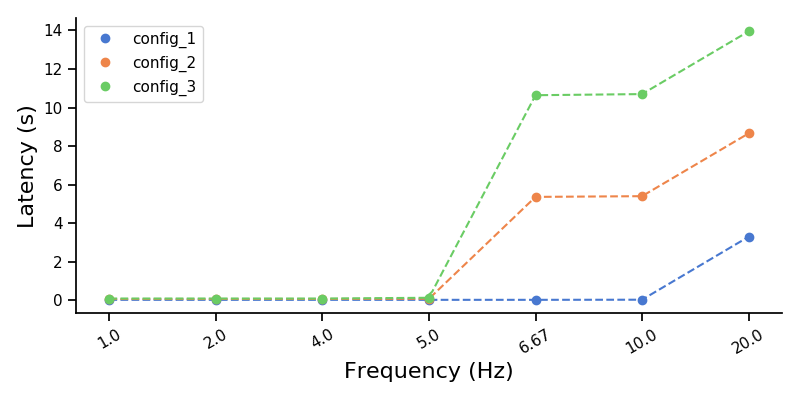
\includegraphics[width = 0.95\textwidth]{images/graphs/ble_latency.png}
    \caption{Latency - Bluetooth Mesh}
    \label{graph:ble_latency}
\end{figure}

\noindent I risultati in maniera dettagliata sono riportati in appendice, nella sezione \nameref{apex:outcomes_ble_mesh}. I valori sono rappresentati con tre cifre decimali al fine di facilitare la lettura. Per le tre metriche in esame sono riportati i valori \textit{medi} con accanto indicato il \textit{margine d'errore} al fine di affermare con una margine di certezza ragionevole l'intervallo che conterrà il valore vero dell'intera popolazione. Nei casi in cui il margine d'errore (\texttt{m\_e}) coincide con il valore $0.0$, vuol dire che esso è talmente piccolo (richiede più valori decimali) e viene approssimato a tale cifra.

\subsubsection{Risultati Approccio Misto}
Con l'introduzione della tecnologia di supporto si è ottenuto un maggiore livello prestazionale a cui però è soggetto un maggior consumo energetico oltre ad un leggero incremento della latenza, dovuta alla determinazione della perdita del pacchetto per poi inviarlo nuovamente. Utilizzando questa configurazione (con l'impiego dello stack Bluetooth Mesh e l'impiego dello stack Wi-Fi) si sono ottenuti i risultati descritti di seguito.\\

\noindent Come accade con la situazione descritta in precedenza, anche in tale circostanza si verifica un calo prestazionale della rete con l'aumentare dei nodi e delle frequenze trasmissive. La differenza di questo calo prestazionale sta proprio nei valori, poiché in tale circostanza il valore più basso (\texttt{conf\_3} - tasso d'invio di \texttt{50 ms}) riscontrato dall'esecuzione dei 5 run di simulazione è $0.924$, mentre con l'impiego della solo tecnologia Bluetooth Mesh, nella medesima situazione, il valore ottenuto è di gran lunga inferiore, ovvero $0.2$ $\pm$ $0.012$ (per maggiori dettagli visualizzare i grafici e le tabelle in appendice).

\begin{figure}[hbt!]
    \centering
    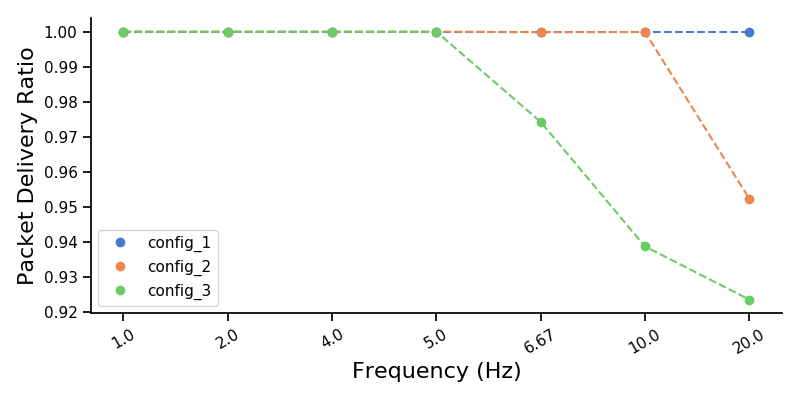
\includegraphics[width = 0.95\textwidth]{images/graphs/ble_wifi_pdr.png}
    \caption{Packed Delivery Ratio - Approccio Misto}
    \label{graph:ble_wifi_pdr}
\end{figure}

\noindent Come anticipato, l'introduzione dell'algoritmo misto introduce una certo ritardo al fine di determinare se un pacchetto effettivamente risulta essere perso oppure, a causa del carico di lavoro elevato con cui la rete sta operando, impiegherà più tempo del previsto per giungere a destinazione e successivamente tornare indietro.\\
L'algoritmo prevede un adeguamento piuttosto lento della soglia, proprio per far fronte ad una situazione del genere. La quale però, analizzando i risultati riportati nel grafico seguente e confrontati con il grafico dell'approccio Bluetooth Mesh (\nameref{graph:ble_latency}), si notano dei valori leggermente più alti. Un confronto immediato può essere eseguito analizzando il grafico relativo alla latenza in appendice, nella sezione \nameref{apex:grafici}.\\
Le curve, distinte in base alla configurazione, in entrambi i grafici presentano un andamento molto simile. Ovvero tendono a discostarsi dalla \texttt{configurazione 1} nel momento in cui si ha un tasso d'invio di \texttt{150 ms}.

\begin{figure}[hbt!]
    \centering
    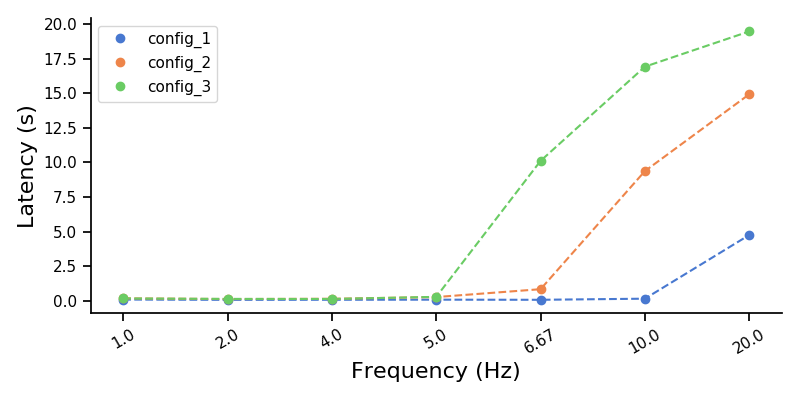
\includegraphics[width = 0.95\textwidth]{images/graphs/ble_wifi_latency.png}
    \caption{Latency - Approccio Misto}
    \label{graph:ble_wifi_latency}
\end{figure}

\noindent Con l'impiego dell'approccio misto, le prestazioni della rete risultano essere nettamente migliori e questo è percepibile analizzando il grafico relativo al goodput. A differenza della situazione verificata con l'altro approccio, qui si ha un andamento pressoché identico per tutte e tre le configurazioni. Garantendo di fatto l'efficacia dell'algoritmo implementato.

\begin{figure}[hbt!]
    \centering
    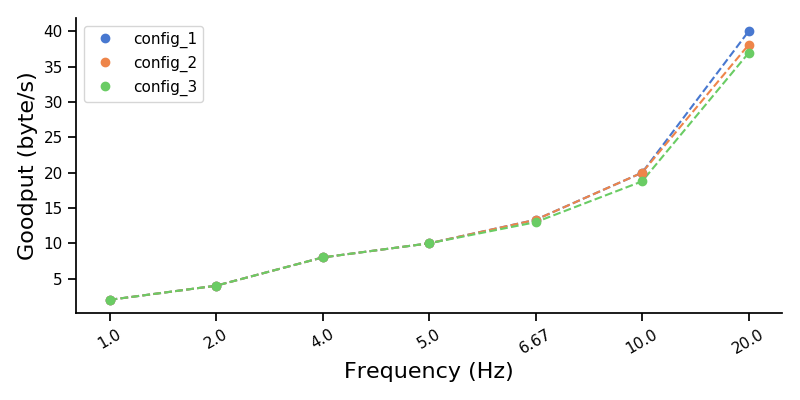
\includegraphics[width = 0.95\textwidth]{images/graphs/ble_wifi_goodput.png}
    \caption{Goodput - Approccio Misto}
    \label{graph:ble_wifi_goodput}
\end{figure}

\noindent Come indicato in precedenza, in appendice, nella sezione \textit{\nameref{apex:grafici}} è possibile osservare i grafici che riportano entrambe le situazioni, al fine di percepire in maniera molto più rapide le differenze e l'efficacia dell'algoritmo in termini prestazionali. I risultati in forma tabellare sono riportare in appendice, nella sezione \nameref{apex:outcomes_ble_wifi_mesh}. 
Solitamente i valori sono rappresentati con tre cifre decimali al fine di semplificare la lettura, ma nei casi in cui risultano essere talmente piccoli che non è possibile rappresentarli correttamente in tale modo, sono rappresentati in notazione scientifica utilizzando due decimali. Questa situazione si verifica con il margine d'errore (\texttt{m\_e}) poiché i valori ottenuti nelle 5 ripetizioni risultano molto simili tra loro. Nel caso in cui il valore è \texttt{0.0} vuol dire che non c'è stata nessuna perdita di pacchetto in tutte le ripetizioni e quindi si ottiene sempre il medesimo valore.\\

\subsubsection{Percentuali impiego tecnologie in fase di trasmissione}
\noindent Analizzando più del dettaglio i file di log ottenuti tramite l'impiego dell'approccio misto è stato possibile distinguere tra i pacchetti aventi esito positivo, quelli andati a buon fine attraverso la tecnologia Bluetooth e quelli per cui è stato necessario ricorrere ad una ritrasmissione e quindi andati a buon fine attraverso la tecnologia Wi-Fi. \\
I grafici proposti di seguito permetteranno di comprendere meglio il comportamento del protocollo. I valori mostrati indicano il comportamento al variare della frequenza, per ogni singola configurazione. L'impiego delle due tecnologie viene indicato attraverso una scala percentuale, calcolata sui pacchetti definiti come ricevuti con successo.

\begin{figure}[hbt!]
    \centering
    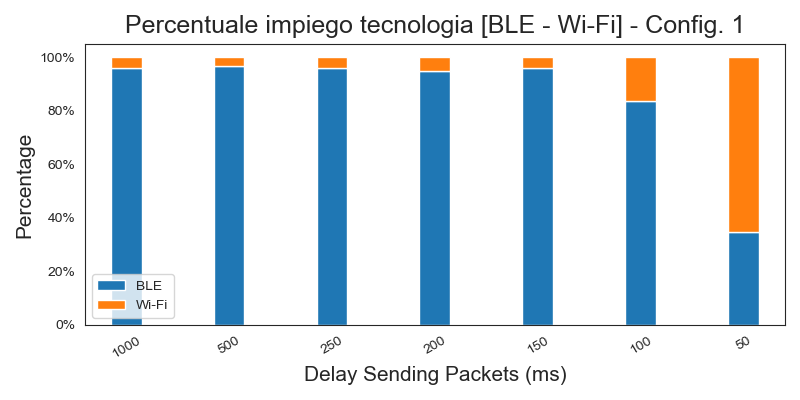
\includegraphics[width = 1\textwidth]{images/graphs/myplot_config_1_title.png}
    \caption{Gestione pacchetti - \texttt{Configurazione 1}}
    \label{graph:mixed_conf_1}
\end{figure}

\noindent Osservando il grafico \ref{graph:mixed_conf_1} relativo alla \texttt{configurazione 1} si può notare un comportamento prettamente omogeneo con le frequenza più basse, ovvero un impiego della tecnologia Wi-Fi quasi inesistente finché non si giunge, in fase di trasmissione, ad una frequenza pari ai 10 Hz (invio di un pacchetto ogni 100 ms). In tale circostanza si avverte un leggero declino prestazionale che viene accentuato notevolmente (più che dimezzato) nel momento in cui si passa alla frequenza più alta utilizzata per i testbed creati.\\
Questo andamento, descritto dal seguente grafico risulta essere quello meno gravoso per la tecnologia Bluetooth Mesh, poiché ci si trova in un contesto molto semplice, ovvero costituito esclusivamente dai nodi mittente e destinatario e quindi senza la presenza di nodi intermedi aventi la funzione di relay, i quali come indicato nei successivi grafici comporteranno dei cali prestazionali alla tecnologia Bluetooth.

\begin{figure}[hbt!]
    \centering
    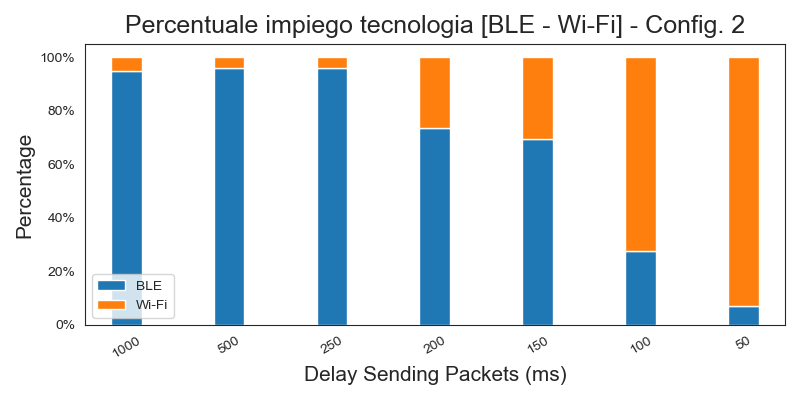
\includegraphics[width = 1\textwidth]{images/graphs/myplot_config_2_title_n.png}
    \caption{Gestione pacchetti - \texttt{Configurazione 2}}
    \label{graph:mixed_conf_2}
\end{figure}

\noindent Osservando il grafico \ref{graph:mixed_conf_2} relativo alla \texttt{configurazione 2} si nota un impiego molto sporadico della tecnologia Wi-Fi, così come accaduto con la \texttt{configurazione 1}, ma questa volta, tale situazione si è verificata finché non si è giunto all'invio dei dati con una frequenza pari a 5 Hz (invio di un pacchetto ogni 200 ms). In quest'ultimo caso, seppur risulta essere più elevato l'impiego della tecnologia Wi-Fi è pur sempre molto inferiore rispetto alla tecnologia predefinita, ovvero comprende il 27\% dei pacchetti trasmessi con successo.\\
Un comportamento molto simile si è verificato anche con una frequenza d'invio di 6.67 Hz (invio di un pacchetto ogni 150 ms), in cui l'impiego della tecnologia Wi-Fi è leggermente più altro del caso precedente, ovvero coincide al 31\%.
Con le due frequenze più alte (10 Hz e 20 Hz), invece, l'impiego della tecnologia Wi-Fi prende il sopravvento rispetto alla tradizionale, con un impiego rispettivamente del 72\% e del 92\%.\\
Questo comportamento era da aspettarselo ed è influenzato proprio dalla presenza di un dispositivo intermedio per consentire la comunicazione tra mittente e destinatario.

\begin{figure}[hbt!]
    \centering
    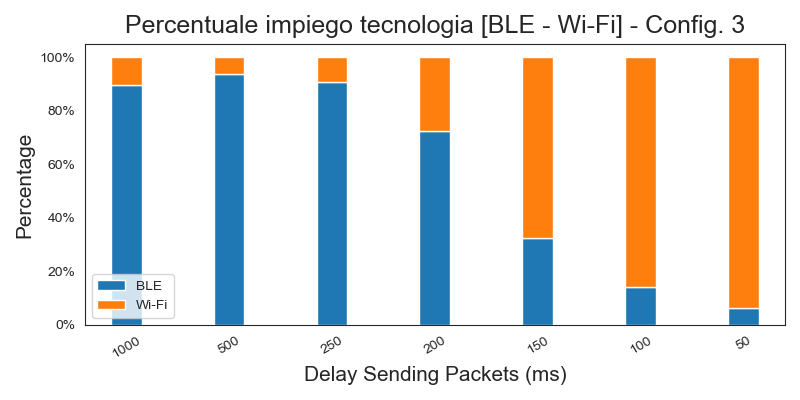
\includegraphics[width = 1\textwidth]{images/graphs/myplot_config_3_title_n.png}
    \caption{Gestione pacchetti - \texttt{Configurazione 3}}
    \label{graph:mixed_conf_3}
\end{figure}

\noindent Osservando il grafico \ref{graph:mixed_conf_3} relativo alla \texttt{configurazione 3} si nota un comportamento molto simile alla \texttt{configurazione 2}, ma con dei valori più bassi in termini di impiego della tecnologia Bluetooth. In questo grafico, dei peggioramenti si avvertono a partire dalle frequenze più basse, proprio perché, nella suddetta configurazione è stato introdotto un altro dispositivo intermedio per garantire la comunicazione tra mittente e destinatario. In questo caso l'inversione relativo alla tecnologia utilizzata maggiormente durante il relativo test avviene a partire dalla frequenza 6.67 Hz, mentre nella \texttt{configurazione 2} è avvenuto a partire dalla frequenza di invio pari a 10 Hz e nella \texttt{configurazione 1}, invece, è avvenuto solo ed esclusivamente con la frequenza di trasmissione più alta, ovvero 20 Hz.\\

\noindent Come ci si aspettava, aumentando la frequenza di trasmissione il numero di pacchetti persi con la tecnologia Bluetooth risulta essere piuttosto elevato e di conseguenza c'è un maggior impiego della tecnologia Wi-Fi, mentre con frequenza molto basse, tendenti ad 1 Hz, l'impiego della tecnologia BLE risulta essere predominante (tabella impiego tecnologie presente in appendice - \ref{tab:table_perc_ble_wifi}).
Come indicato dai grafici inerenti le metriche calcolate (principalmente il grafico relativo al PDR), anche questi ultimi grafici mostrano come all'aumentare della frequenza d'invio e con l'introduzione dei nodi intermedi, ovvero con l'aumentare della distanza tra mittente e destinatario, le prestazioni della rete tendono a diminuire, ovvero si avverte un maggior numero di perdite di pacchetti Bluetooth e quindi la necessità di una loro ritrasmissione, che avviene a seguito di un'analisi eseguita dall'algoritmo dinamico descritto nei capitoli precedenti e attuata per mezzo della tecnologia Wi-Fi.\\

\noindent Un grafico riassuntivo ed una tabella che espone i valori percentuali relativi al comportamento del protocollo, in cui è mostrata l'alternanza tra le due tecnologie nelle tre configurazione è presente in appendice, nella sezione \textit{\nameref{apex:grafici_packets}}.
